% Standalone YOLO11 pipeline diagram for the end-sem presentation.
% Compile with pdflatex (or use Overleaf), then export the PDF as a PNG
% and paste it into the slide. Same diagram as in the main report.
\documentclass[border=10pt]{standalone}
\usepackage{tikz}
\usetikzlibrary{shapes.geometric, arrows.meta, positioning, calc}
\begin{document}
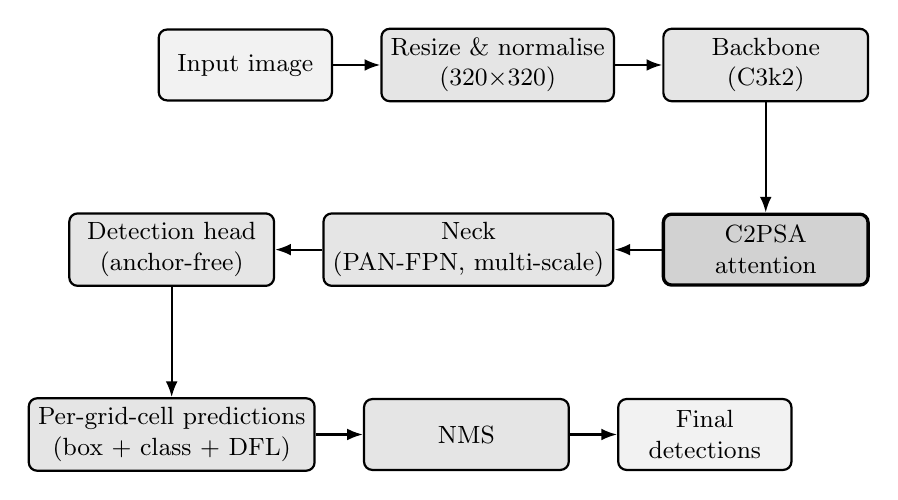
\begin{tikzpicture}[
    font=\small,
    node distance=8mm and 6mm,
    every node/.style={align=center},
    io/.style   ={rectangle, rounded corners=3pt, draw, thick,
                  minimum width=22mm, minimum height=9mm, fill=gray!10},
    proc/.style ={rectangle, rounded corners=3pt, draw, thick,
                  minimum width=26mm, minimum height=9mm, fill=gray!20},
    attn/.style ={rectangle, rounded corners=3pt, draw, very thick,
                  minimum width=26mm, minimum height=9mm, fill=gray!35},
    arr/.style  ={-{Latex[length=2mm]}, thick}
]
% Row 1
\node[io]   (img)     {Input image};
\node[proc, right=of img]  (pre)     {Resize \& normalise\\(320$\times$320)};
\node[proc, right=of pre]  (back)    {Backbone\\(C3k2)};

% Row 2
\node[attn, below=14mm of back]  (attn)    {C2PSA\\attention};
\node[proc, left=of attn]        (neck)    {Neck\\(PAN-FPN, multi-scale)};
\node[proc, left=of neck]        (head)    {Detection head\\(anchor-free)};

% Row 3
\node[proc, below=14mm of head]  (pred)    {Per-grid-cell predictions\\(box + class + DFL)};
\node[proc, right=of pred]       (nms)     {NMS};
\node[io,   right=of nms]        (out)     {Final\\detections};

% Arrows row 1
\draw[arr] (img)  -- (pre);
\draw[arr] (pre)  -- (back);
\draw[arr] (back.south) -- ++(0,-3mm) -| (attn.north);
\draw[arr] (attn) -- (neck);
\draw[arr] (neck) -- (head);
\draw[arr] (head.south) -- ++(0,-3mm) -| (pred.north);
\draw[arr] (pred) -- (nms);
\draw[arr] (nms)  -- (out);
\end{tikzpicture}
\end{document}
